%Carthage Physics Senior Thesis
%Author: Aaron Scheets

\documentclass[twocolumn,12pth]{article}
\usepackage[hmargin={1.25in,0.75in},bmargin=1in,tmargin=1in]{geometry} 
\usepackage{setspace}
\usepackage{url}
\usepackage{syntonly}
\usepackage[ampersand]{easylist}

\usepackage{natbib}

\usepackage{amsmath}
\usepackage{mathtools}
\usepackage{gensymb}
\usepackage{amssymb}
\usepackage{float}
\providecommand{\e}[1]{\ensuremath{\times 10^{#1}}}

\usepackage{graphicx}
\usepackage{caption}


\title{Writing A Fluid Solver From First Principles (Introduction/Mathematical Model)}

\author{Aaron Scheets}

\onecolumn

\begin{document}

%\doublespacing

\maketitle

\section{Introduction}

This thesis is an investigation of the components of a ``fluid solver''.
Some of the most, exciting, beautiful, and complicated processes in nature are problems of fluid mechanics.
There are extraordinary fluid phenomena to model from the scale of the plume of steam coming from your cup of coffee in the morning (and even smaller), to the dynamics of ocean currents (and even larger).
Words can hardly do these flows justice, which is why visualization of flows is so important in fluid dynamics.
The only problem is, the math behind these exciting flows usually can't be solved analytically. 
We can make simplifications on systems to solve them analytically, or we can setup the problem in such a way that a computer can give us an approximate answer by making a very large number of calcuations.
The goal of my thesis research was to investigate the process of modeling a dynamic fluid mathematically and then using computational methods to visualize that fluid.
Visualizing a fluid means solving for the velocity, pressure or temperature of that fluid.
The dynamic fluid I have modeled is an \textit{incompressible} fluid, like water, flowing in a pipe. 
I chose the case of incompressible flow in a pipe because, making certain simplifications, incompressible flow in a pipe can be solved for analytically. 

\subsection{Fluid Modeling Process}

For the sake of consistency and organization in the midst of the somewhat intimidating task of writing a fluid solver, it is helpful to establish an outline of our approach to the problem.
So, imagine someone places a clear pipe through which water is flowing in front of you, and asks you: What is the velocity of the water in the pipe?
The approach you might take to answering this question depends on the accuracy demanded by the person asking for the velocity.
Determining the velocity in the pipe will involve some combination of mathematical analysis and experimental verification.
It would make sense, if one were to derive a mathematical expression for the fluid velocity in the pipe, to construct an experiment which could verify the correctness of the model.
When replication of the fluid process cannot be easily done in the lab, or when the measurement of the fluid properties would interfere with the flow, computational visualizations take the place of physical experiment.
The following are a basic overview of the computational modeling process:
\vspace{2mm}

\begin{easylist}[enumerate]
& Mathematical model
& Discretization method
& Analyze validitiy of discretization method
& Solve system using computer
& Visualize and anaylze results
\end{easylist}

\vspace{2mm}
The starting point of a computational fluid dynamics study is the mathematical model.
Once one has come up with a mathematical model for the fluid in question, a discretization scheme is applied to the model.
Discretization schemes express the continuous equations of the model in a form that can be solved by a computer.
After a discretization scheme has been chosen, one must analyze the validity of the scheme in the context of the fluid in question: does the scheme violate any of the physics governing the fluid?
After the scheme has been validated, hopefully the scheme can be solved by a computer to produce a data set for the velocity and pressure of the fluid.
The velocity vector field and pressure scalar field must then be visualized using graphical software for further analysis.
The rest of this document will present what each of these components entails and how the component was applied to incompressible, unsteady, fluid flow in a pipe.

\section{Mathematical Model}

\subsection{What is a fluid?}

The first question one might have is, what is a fluid?
A fluid is a substance without resistance to \textit{shear} forces.
Imagine a cube of some particular substance, and consider the top and bottom face of that cube in particular.
Apply a force tangential to the top face and a separate force tangential to the bottom face and the result is shear.
Now, picture two cubes resting on a table; one a solid cube of ice and the other a cube of water.
Were you to give each cube a nudge near the top face, the ice cube would retain its shape and maybe move along the table.
The result of nudging the fluid cube would be continous \textit{deformation}, the cube would lose its shape as the water spreads over the table.
The deformation the fluid undergoes is due to the fluid's lack of resistance to shear, which is a result of the molecular properties of the fluid.
The attraction between molecules within the solid is greater than those found in the fluid.
Gases are also fluids as they show no resistance to sideways forces.

\subsection{Fluid Adjectives}

Previously I mentioned the extensive nature of fluid mechanics and that I modeled \textit{incompressible} fluid flow.
An incompressible fluid, like water, is a fluid whose density is constant, in contrast to a compressible fluid, like air, whose density is not constant.
These adjectives describe physical characteristics of the differing fluids.
Specifying a fluid using these adjectives gives us a sense of what equations should be used to model the fluid, and what assumptions can be made to simplify those equations.
Figure ? depicts the divisions in physical characteristics made when considering a fluid.
Going right through this chart, I can classify the fluid subject of my model: liquid, incompressible, unsteady, viscous, rotational, and two-dimensional!
These characteristics dictate which equations I can and should use to model the fluid.
Since I am modeling an incompressible fluid, I will be using the \textit{Navier-Stokes Equations}, if the fluid were a compressible gas, I would instead use Euler's equations.

\subsubsection{Newton's Second Law Applied to a Control Volume}

We can obtain a general notion for what the general equations of fluid motion should consist of by applying Newton's Second Law to a control volume of fluid.
Newton's second law states that the mass times acceleration of a system is equal to the net force applied to that system:

\begin{equation*}
m\vec{a} = \sum{F_{system}}
\end{equation*}

Another way of expressing Newton's Second is equating the rate of change of momentum with respect to time of the system to the sum of the forces on that system:

\begin{equation}
\frac{d{\vec{p}}}{dt} = \sum F_{system}
\end{equation}

These expressions are Newton's Second Law as applied to a \textit{system}.
In the case of fluids a system is defined as a specific group of fluid particles: ``the volume, pressure, and temperature of the system can change but the system, that is, the identity of mass, does not change''. \cite{Granger1995}
This is also the case with rigid bodies like point masses, but in that case it is not usually something worth distinguishing.
In contrast to a system, is the \textit{control volume}, which is a definite volume of space, established by a set of surfaces, through which fluid mass can flow.
We can see why the difference between a system and a control volume has to be made clear if we remember that we are trying to figure out the velocity of the fluid within some larger volume, in this case the pipe.
Were we to apply Newton's Second Law as is, we would have to keep track of a set of masses as they pass through the pipe.
One can imagine how hard it woud be to mathematically model the path of one particular chunk of flowing water.
It would be much easier to divide our pipe into a set of definite volumes and apply the control volume approach at each of these volumes by observing the mass passing through the volume surfaces.
That being said, we have to come up with a form of Newton's Second Law that applies to a control volume rather than a system.

\subsubsection{Reynolds' Transport Theorem}

In the last section, we were interested in finding the derivative of momentum with respect to time for use in Newton's Second Law.
To find the derivative of momentum, we first want to find an equation for the derivative of any property of the fluid.
Momentum is a property of our fluid, and if we can find a generic fluid derivative, it can be applied to momentum just as well.
In order to find this fluid derivative, we must think about how properties change within a fluid.
Remember, we are interested in applying Newton's Second Law to a control volume.
For each property we are considering, and the derivative of that property, there will be a corresponding control volume.

Consider a pipe with water flowing through it, and imagine dumping a bucket of microbeads into the water at the front of the pipe.
We first shall consider the total number of beads in the pipe and how this value changes with time.
When considering the total number of beads in the pipe, our control volume of interest is the pipe itself.
To find the total number of beads in the pipe at a given moment, we integrate the density of beads throughout the pipe, $\rho$ over the entire volume of the pipe, $V$:

\begin{equation}
\int_{V} \rho dV
\end{equation}

Let's say we have run out of beads to pour into the pipe.
There is now a distinct number of beads in the pipe, and the only way that number can change is if the beads exit the pipe through some surface.
At the end of our pipe there is an outlet through which the water and beads are flowing.
This outlet can be described by a particular surface area vector $\mathbf{S}$, which consists of a particular area magnitude $S$ and a vector normal to the surface $\mathbf{n}$.
We can describe the number of beads exiting the pipe through this surface as a flux.
The flux takes into account the velocity of the beads in the direction of the surface, $\mathbf{n}$, and the bead density of the water passing through the surface:

\begin{equation}
\int_S \rho \mathbf{v} \cdot \mathbf{n} dS
\end{equation}

Since the only way the beads can leave the pipe is through this outlet, we can safely equate the rate of change of the total number of beads in the pipe to the flux of beads through the outlet $S$:

\begin{equation}
\int_S \rho \mathbf{v} \cdot \mathbf{n} dS = - \frac{d}{dt} \int_{V} \rho dV
\label{eq:rtt}
\end{equation}

Notice the flux of beads through the surface is equal to negative the time rate of change of beads in the pipe because beads are exiting the pipe at this surface.
One should find the unit of the flux through $S$ is beads per second.
This is equivalent to what we would expect for the derivative of the total number of beads in the pipe.
The expression we just found is the integral form of what is known as the \textit{Reynolds' Transport Theorem} in the context of fluid mechanics.
Given some particular control volume, and the density of some property within that volume, $\rho$, the Reynolds' Transport Theorem expresses the time rate of change of $\rho$.

Consider Gauss' Divergence theorem:

\begin{equation}
\int_S \mathbf{F} \cdot d\mathbf{a} = \int_V div(\mathbf{F}) dV
\end{equation}

\begin{equation}
\int_S \rho \mathbf{v} \cdot \mathbf{n} dS = \int_V div(\mathbf{\rho{v}}) dV
\end{equation}

Gauss's theorem relates the flux of a particular vector field over a surface enclosing a volume to the divergence of that vector quantity within the volume.
Applying Gauss's theorem to the transport theorem (\ref{eq:rtt}) we are left with:

\begin{equation}
\int_V div(\mathbf{\rho{v}}) dV = - \frac{d}{dt} \int_{V} \rho dV
\label{eq:rtt2}
\end{equation}

This expression involves two integrals, both over some volume $V$.
As long as $\rho$ is continuous over $V$, the derivative of the integral will be equal to the integral of the derivative (move the derivative inside the integral).
As long as our volume $V$ is much larger than the scale of individual fluid particles, we can assume our expression (\ref{eq:rtt2}) holds for any volume (drop the integral over $V$).
Thus, we are left with the differential form of the Reynolds Transport Theorem:

\begin{equation*}
div(\rho \mathbf{v}) = -\frac{\partial{\rho}}{\partial{t}}
\end{equation*}

\begin{equation}
\frac{\partial{\rho}}{\partial{t}} + div(\rho \mathbf{v}) = 0
\label{eq:der}
\end{equation}

This is the expression for the derivative of a fluid property, given that property is in the form of a density, $\rho$.


\subsubsection{Conservation of Mass, Momentum}

In the previous section, we found the derivative of the density of a property in a fluid.
We were originally interested in finding the derivative of momentum in a fluid for use with Newton's Second Law.
The next step would then be to express the momentum of our fluid as a density.
The density of a particular property is the value of that property per some volume.
It is helpful to first think of the density of mass within the fluid.
Mass per volume is a concentration we are familiar with, and it is a density we can measure.
Since we can measure the mass per volume of a liquid, we will designate $\rho$ for this particular type of density:

\begin{equation}
\rho = \frac{\mathrm{mass}}{\mathrm{volume}}
\end{equation}

It is important to remember that in the previous section when we derived the fluid derivative, $\rho$ represented a generic density: the quantity of any property per volume.
Now $\rho$ is specifically the mass density: the quantity of mass per volume.
Momentum is the product of mass and velocity, $mv$.
To find the density of momentum within our fluid, we divide $mv$ by volume.

\begin{equation}
\mathrm{density \,\, of \,\, momentum} = \frac{\mathrm{mass} \cdot \mathrm{velocity}}{\mathrm{volume}}
\end{equation}

Using our new definition of $\rho$ as the mass density, we can rewrite the density of momentum in the fluid as $\rho$ times velocity:

\begin{equation}
\mathrm{density \,\, of \,\, momentum} = \rho{v}
\end{equation}

Recalling our fluid derivative from the previous section (\ref{eq:der}), we can now write the derivative of mass (\ref{eq:massDer}), and the derivative of momentum (\ref{eq:momDer}) within our fluid:

\begin{equation}
\frac{\partial{\rho}}{\partial{t}} + div(\rho \mathbf{v})
\label{eq:massDer}
\end{equation}

\begin{equation}
\frac{\partial{\rho}\mathbf{v}}{\partial{t}} + div(\rho \mathbf{vv})
\label{eq:momDer}
\end{equation}

The conservation of mass allows us to equate the mass derivative to zero (\ref{eq:massDer2}): mass will neither be created nor destroyed. \cite{Ferziger2002}
Returning to Newton's Second Law, we will equate the momentum derivative to the sum of forces on the fluid.

\begin{equation}
\frac{\partial{\rho}}{\partial{t}} + div(\rho \mathbf{v}) = 0
\label{eq:massDer2}
\end{equation}

\begin{equation}
\frac{\partial{\rho}\mathbf{v}}{\partial{t}} + \mathbf{v} \cdot grad(\rho \mathbf{v}) = \sum{\mathrm{fluid \,\, forces}}
\label{eq:momDer2}
\end{equation}

Both of the conservation equations (\ref{eq:massDer2}), (\ref{eq:momDer2}) are vector partial differential equations and are perhaps a little easier to understand when written as a set of component equations.
The velocity vector function, $\mathbf{v}$, has $x$, $y$, and $z$ components of velocity $u$, $v$, and $w$, respectively.
Notice how the density, $\rho$ has been factored out of the partials; we can do this because our simulated fluid is incompressible with constant density (constant density in time and space).

\begin{equation}
\frac{\partial{u}}{\partial{t}} + u\frac{\partial{u}}{\partial{x}} + v\frac{\partial{u}}{\partial{y}} + w\frac{\partial{u}}{\partial{z}} = \frac{1}{\rho}\mathbf{F}_x
\label{eq:momComps}
\end{equation}

\begin{equation*}
\frac{\partial{v}}{\partial{t}} + u\frac{\partial{v}}{\partial{x}} + v\frac{\partial{v}}{\partial{y}} + w\frac{\partial{v}}{\partial{z}} = \frac{1}{\rho}\mathbf{F}_y
\end{equation*}

\begin{equation*}
\frac{\partial{w}}{\partial{t}} + u\frac{\partial{w}}{\partial{x}} + v\frac{\partial{w}}{\partial{y}} + w\frac{\partial{w}}{\partial{z}} = \frac{1}{\rho}\mathbf{F}_z
\end{equation*}

You might have noticed that the form of the divergence term changed from equation (\ref{eq:momDer}) to (\ref{eq:momDer2}).
To see why, we should apply the chain rule to the divergence term in equation (\ref{eq:momDer}), but in the context of one of the component equations, $v_i$. \cite{Ferziger2002}

\begin{equation}
div(\rho \mathbf{v}v_i) = v_i div(\rho\mathbf{v}) + \rho\mathbf{v} \cdot grad(v_i)
\end{equation}

Using equation (\ref{eq:massDer2}), which expresses the conservation of mass in our system, the first term on the left in the above equation is equal to zero.
Thus, our original divergence of momentum term can be simplified:

\begin{equation}
div(\rho \mathbf{vv_i}) = \rho\mathbf{v} \cdot grad(v_i)
\end{equation}

We are one step closer to the equations of fluid motion.
We have found the complete form for the conservation of mass, and the rate of change of momentum within our fluid.
Next, we must determine the forces that act on the fluid control volume.

\subsubsection{Fluid Forces}

One can mathematically describe forces within a fluid by isolating a cubic volume of fluid and considering the possible ways forces can be applied to that volume. 
We are interested in finding the forces on a fluid for use in Newton's Second Law.
A force we know will act on the fluid is gravity.
In fluid mechanics, forces are separated into two categories, \textit{body forces} and \textit{surface forces}.
Gravity is a body force because we determine the magnitude of the force by integrating over the entire volume of fluid.
The force of gravity acts equally upon every particle within the fluid.
Normally we would find the force of gravity by multiplying mass by the acceleration due to gravity, g.
In the case of our a control volume within the fluid, where we are interested in the density of properties, mass is once again $\rho$.
Thus, the force of gravity acting on a control volume in the fluid is the following:

\begin{equation}
\mathbf{F}_g = \rho\mathbf{g}
\label{eq:grav}
\end{equation}

The acceleration vector due to gravity doesn't always have to be in the y-direction, so in the general case we consider all components of the force due to gravity.
Surface forces act upon the surface of the volume and diminish in magnitude moving away from the surface of the fluid.
Pressure is an example of a surface force; pressure acts normal to the surface of the fluid.
The component of force tangential to the surface of a fluid is known as shear force.
The shear force is associated with the viscosity of the fluid.
In the context of surface forces, since we are integrating over a surface, pressure force and shear force are more relevant as \textit{stresses}.
A stress is defined as a force per area.
The pressure stress is denoted by $\sigma_{ii}$, see Figure \ref{fig:stresses}.
The shear stress is listed as $\tau_{ij}$.
The subscript $i$ indicates the direction of the normal vector of the particular surface the force is acting on.
The subscript $j$ indicates the direction in which the force is acting.
For example, consider the shear stress on face 2 of the fluid volume, $\tau_{yx}$.
The first index is $y$ because the normal vector of face 2 points in the y direction.
The second index is $x$ because the stress, $\tau_{yx}$ acts in the x direction.

\begin{figure}
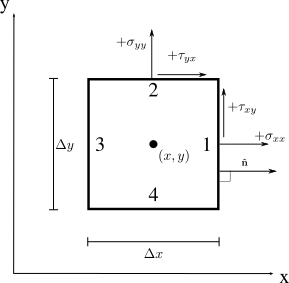
\includegraphics[width=3.0in]{stresses.png}
\centering
\captionof{figure}{}
\label{fig:stresses}
\end{figure}

We would like to express the x, y, and z component of force on the fluid volume due to the surface stresses.
To do this, sum up all of the stresses in the x, y, or z, direction.
Let us consider the surface forces on our fluid volume in the x direction.
Our entire mathematical model rests on data at a set of points.
That is, we know the value of the stresses at the point $(x,y)$, but the surface forces act some distance away from $(x,y)$.
If we assume the surface stresses are constant throughout the fluid, this is no problem, otherwise, we have to take into account the spatial variation of the surface stresses.
The surface force is calculated by multiplying the surface stress by the area over which it acts.
Taking all of this into account, the surface forces acting in the x, y, and z direction, for a 3-dimensional volume of fluid are the following:

\begin{equation}
\mathbf{F}_{S,x} = dxdydz \bigg( \frac{\partial{\sigma_{xx}}}{\partial{x}} + \frac{\partial{\tau_{yx}}}{\partial{y}} + \frac{\partial{\tau_{zx}}}{\partial{z}} \bigg)
\label{eq:sf}
\end{equation}

\begin{equation*}
\mathbf{F}_{S,y} = dxdydz \bigg( \frac{\partial{\tau_{xy}}}{\partial{x}} + \frac{\partial{\sigma_{yy}}}{\partial{y}} + \frac{\partial{\tau_{zy}}}{\partial{z}} \bigg)
\end{equation*}

\begin{equation*}
\mathbf{F}_{S,z} = dxdydz \bigg( \frac{\partial{\tau_{xz}}}{\partial{x}} + \frac{\partial{\tau_{yz}}}{\partial{y}} + \frac{\partial{\sigma_{zz}}}{\partial{z}} \bigg)
\end{equation*}

We have now expressed the body and surface forces we might find applied to a 3-dimensional volume of fluid. 
The only body force we are considering is gravity, (\ref{eq:grav}).
We just found the x, y, and z components of the surface forces, due to pressure and viscous forces, (\ref{eq:sf}).
Previously, we found the rate of change of the momentum in the fluid, (\ref{eq:momComps}).
Now, to completely express the conservation of momentum in the fluid, we need to substitute the net x, y, and z forces on the fluid into equation (\ref{eq:momComps}).
For brevity, I will only include what this would look like for the x-direction.

\begin{equation}
\frac{\partial{u}}{\partial{t}} + u\frac{\partial{u}}{\partial{x}} + v\frac{\partial{u}}{\partial{y}} + w\frac{\partial{u}}{\partial{z}} = g_x + \frac{1}{\rho} \bigg(\frac{\partial{\sigma_{xx}}}{\partial{x}} + \frac{\partial{\tau_{yx}}}{\partial{y}} + \frac{\partial{\tau_{zx}}}{\partial{z}} \bigg)
\label{eq:momCons}
\end{equation}

Now, let us think about the equations we have available to us, and the number of unknowns in the system.
We have one equation expressing the conservation of mass, (\ref{eq:massDer2}), and three equations from the three component vector equation expressing the conservation of momentum, (\ref{eq:momCons}).
We will set the density of the fluid, so that is not an unknown.
We do not know the value for the three components of the velocity $\mathbf{v}$, and we do not know the value of the surface stresses $\sigma_{ii}$ and $\tau_{ij}$.
The system is underdetermined, there are too many unknowns for the number of equations.


\subsubsection{Navier-Stokes Equations}

The Navier-Stokes equations express the motion of a Newtonian fluid.
A Newtonian fluid is one in which the stresses and velocity derivatives are linearly related.
Below are the relations between the pressure stresses and the velocity derivatives.

\begin{equation}
\sigma_{xx} = -p + 2\mu\frac{\partial{u}}{\partial{x}}
\label{eq:norms}
\end{equation}

\begin{equation*}
\sigma_{yy} = -p + 2\mu\frac{\partial{v}}{\partial{y}}
\end{equation*}

\begin{equation*}
\sigma_{zz} = -p + 2\mu\frac{\partial{w}}{\partial{z}}
\end{equation*}

The shear stresses are also linearly related to the velocity derivatives.

\begin{equation}
\tau_{xy} = \tau_{yx} = \mu\bigg(\frac{\partial{u}}{\partial{y}} + \frac{\partial{v}}{\partial{x}}\bigg)
\label{eq:tangs}
\end{equation}

\begin{equation*}
\tau_{yz} = \tau_{zy} = \mu\bigg(\frac{\partial{v}}{\partial{z}} + \frac{\partial{w}}{\partial{y}}\bigg)
\end{equation*}

\begin{equation*}
\tau_{zx} = \tau_{xz} = \mu\bigg(\frac{\partial{w}}{\partial{x}} + \frac{\partial{u}}{\partial{z}}\bigg)
\end{equation*}

The Navier-Stokes equations also assume that the fluid is incompressible, and isothermal.
An incompressible fluid has constant, uniform density throughout.
An isothermal fluid has constant, uniform temperature throughout.
The divergence of the velocity in an incompressible fluid will be zero.

\begin{equation}
\bigg( \frac{\partial{u}}{\partial{x}} + \frac{\partial{v}}{\partial{y}} + \frac{\partial{w}}{\partial{z}}  \bigg) = \nabla \cdot  \mathbf{v} = 0 \,\, (\mathrm{incompressibility \,\, condition})
\label{eq:ic}
\end{equation}

These values for the pressure and shear stresses, based on the assumptions we are making about the fluid, are known as \textit{constitutive relations}.
Substituting the constitutive relations into the momentum component equations (\ref{eq:momCons}) derived in the previous section can eliminate a few of the unknowns.
Making this substitution equates to taking the partial derivative of the stresses just defined, (\ref{eq:norms}), (\ref{eq:tangs}).

\begin{equation}
\bigg(\frac{\partial{\sigma_{xx}}}{\partial{x}} + \frac{\partial{\tau_{yx}}}{\partial{y}} + \frac{\partial{\tau_{zx}}}{\partial{z}} \bigg) = -\frac{\partial}{\partial{x}}p + 2\mu\frac{\partial^2u}{\partial{x}^2} + \mu\bigg(\frac{\partial^2u}{\partial{y}^2} + \frac{\partial^2v}{\partial{y}\partial{x}} \bigg) + \mu\bigg(\frac{\partial^2w}{\partial{z}\partial{x}} + \frac{\partial^2u}{\partial{z}^2} \bigg)
\end{equation}

The shear stress terms can be simplified using the incompressibility condition.
First, split the $2\mu\frac{\partial^2u}{\partial{x}^2}$ term into two $\mu\frac{\partial^2u}{\partial{x}^2}$ terms.
Then, grouping the partials into factors of $\mu$ as such: 

\begin{equation*}
= -\frac{\partial}{\partial{x}}p + \mu \bigg( \frac{\partial^2u}{\partial{x}^2} + \frac{\partial^2u}{\partial{y}^2} + \frac{\partial^2u}{\partial{z}^2} \bigg) + \mu \bigg( \frac{\partial^2u}{\partial{x}^2} + \frac{\partial^2v}{\partial{y}\partial{x}} + \frac{\partial^2w}{\partial{z}\partial{x}}  \bigg)
\end{equation*}

The rightmost term in this expression can be written as the product of $\mu\frac{\partial}{\partial{x}}$ and the divergence of the velocity, $\nabla \cdot \mathbf{v}$.
From the incompressibility condition (\ref{eq:ic}), this product is equal to zero.

\begin{equation*}
\mu \bigg( \frac{\partial^2u}{\partial{x}^2} + \frac{\partial^2v}{\partial{y}\partial{x}} + \frac{\partial^2w}{\partial{z}\partial{x}}  \bigg) = \mu \frac{\partial}{\partial{x}} \bigg( \frac{\partial{u}}{\partial{x}} + \frac{\partial{v}}{\partial{y}} + \frac{\partial{w}}{\partial{z}}  \bigg) = 0
\end{equation*}

We are left with the following as the surface forces for the x component of the momentum equations.

\begin{equation}
-\frac{\partial}{\partial{x}}p + \mu \bigg( \frac{\partial^2u}{\partial{x}^2} + \frac{\partial^2u}{\partial{y}^2} + \frac{\partial^2u}{\partial{z}^2} \bigg)
\end{equation}

This expression accounts for the surface forces, pressure and viscous forces, in the fluid.
This simplified form of the surface forces came about from the assumptions made regarding the fluid; the fluid is Newtonian, incompressible, and isothermal.
Substituting the simplified form into the x component of the momentum equations:

\begin{equation}
\frac{\partial{u}}{\partial{t}} + u\frac{\partial{u}}{\partial{x}} + v\frac{\partial{u}}{\partial{y}} + w\frac{\partial{u}}{\partial{z}} = g_x -\frac{\partial}{\partial{x}}p + \mu \bigg( \frac{\partial^2u}{\partial{x}^2} + \frac{\partial^2u}{\partial{y}^2} + \frac{\partial^2u}{\partial{z}^2} \bigg)
\end{equation}

This is just one of three component equations maintaining the conservation of momentum.
All three of the equations can be bundled into one using vector notation.

\begin{equation}
\rho(\frac{\partial}{\partial{t}} \mathbf{v} + (\mathbf{v} \cdot \nabla)\mathbf{v} = \rho\mathbf{g} - \nabla{p} + \mu\nabla^2{\mathbf{v}}
\end{equation}

The three component equations of this vector, partial differential equation are what makes up the \textit{Navier Stokes Equations}.
We have derived the equations based upon Newton's Second Law applied to a control volume of fluid.
The left side of the vector equation accounts for the mass 

Explanation of the incompressibility condition pg. 180 purcell

\bibliographystyle{plainnat}
\nocite{*}
\bibliography{library.bib}

\end{document}

